\documentclass[compress]{beamer}

\providecommand{\docroot}{../..}

\input{\docroot/../lib/doc/pkg/beamer}
\input{\docroot/../lib/doc/pkg/beamer_flat_style}
\input{\docroot/../lib/doc/math/operators}

\graphicspath{{\docroot/img/}}

\deftranslation[to=russian]{Theorem}{Теорема}
\deftranslation[to=russian]{theorem}{Теорема}

\title{Нечетные моды\\ сферических гравитационных волн}
\author[Василевский~А.В.]{
    Василевский~А.В. \\[\baselineskip]
    {\footnotesize Научный руководитель: Бурланков~Д.Е.}
}
\institute[ННГУ]{Нижегородский университет им. Н.И.~Лобачевского}
\date{2018}

\begin{document}

    %
    %
    %
    %%%%%%%%%%%%%%%%%%%%%%%%%%%%%%%%%%%%%%%%%%%%%%%%%%%%%%%%%%%%%%%%%%%%%%%
    %                            FRAME                                    %
    %%%%%%%%%%%%%%%%%%%%%%%%%%%%%%%%%%%%%%%%%%%%%%%%%%%%%%%%%%%%%%%%%%%%%%%
    %
    %
    %

    \frame[plain]{\titlepage}

    %
    %
    %
    %%%%%%%%%%%%%%%%%%%%%%%%%%%%%%%%%%%%%%%%%%%%%%%%%%%%%%%%%%%%%%%%%%%%%%%
    %                            FRAME                                    %
    %%%%%%%%%%%%%%%%%%%%%%%%%%%%%%%%%%%%%%%%%%%%%%%%%%%%%%%%%%%%%%%%%%%%%%%
    %
    %
    %

    \begin{frame}\frametitle{Постановка задачи}

        \begin{equation*}
            h^{(o)} = \begin{pmatrix}0&0&h_{13}\\0&0&h_{23}\\h_{13}&h_{23}&0\end{pmatrix}
        \end{equation*}

        \begin{itemize}
            \item Получение аналитических решений для нечетной гармоники сферических гравитационных волн в пустом пространстве.
            \item Описание диаграмм направленности, плотности и потока энергии.
        \end{itemize}

    \end{frame}

    %
    %
    %
    %%%%%%%%%%%%%%%%%%%%%%%%%%%%%%%%%%%%%%%%%%%%%%%%%%%%%%%%%%%%%%%%%%%%%%%
    %                            FRAME                                    %
    %%%%%%%%%%%%%%%%%%%%%%%%%%%%%%%%%%%%%%%%%%%%%%%%%%%%%%%%%%%%%%%%%%%%%%%
    %
    %
    %

    \begin{frame}\frametitle{Квадратичный лагранжиан}

        Метрика искривленного пространства в первом приближении~--- метрика Минковского плюс малые поправки:
        %
        \begin{equation*}
            g_{ij} = \gamma_{ij} + h_{ij}, \qquad h_{00} = 1, \quad h_{0i} = -V_i .
        \end{equation*}

        Квадратичный лагранжиан:
        %
        \begin{equation}\begin{gathered}\label{eq:lagr}
            \mathcal{L}^{(2)} = \frac{1}{8} \qty(
                \gamma^{ij}\gamma^{kl} (E_{ik}E_{jl} - E_{ij}E_{kl}) + B_i^j B_j^i
            ) \sqrt{\gamma} , \\
            E_{ij} = \dot{h}_{ij}, \quad
            B^i_m = (\Opsr{h})^i_m = \varepsilon^{ikl} h_{mk;l}, \quad
            \varepsilon^{ikl} = \flatfrac{1}{\sqrt{\gamma}}.
        \end{gathered}\end{equation}

    \end{frame}

    %
    %
    %
    %%%%%%%%%%%%%%%%%%%%%%%%%%%%%%%%%%%%%%%%%%%%%%%%%%%%%%%%%%%%%%%%%%%%%%%
    %                            FRAME                                    %
    %%%%%%%%%%%%%%%%%%%%%%%%%%%%%%%%%%%%%%%%%%%%%%%%%%%%%%%%%%%%%%%%%%%%%%%
    %
    %
    %

    \begin{frame}\frametitle{Уравнения динамики}

        Возмущения $h_{ij}$ находятся из уравнений динамики:
        %
        \begin{equation*}
            \fdv{\mathcal{L}^{(2)}}{h_{ij}} = 0, \quad
            \fdv{\mathcal{L}^{(2)}}{V_i} = 0 .
        \end{equation*}

        Можно показать, что они сводятся к
        %
        \begin{equation}\label{eq:breq}
            \Opbr{h} = \ddot{h} ,
        \end{equation}
        %
        где
        %
        \begin{equation*}
            \Opbr{h} = \Opsr(\Opsr{h})
        \end{equation*}

        Уравнение \autoref{eq:breq} допускает \textit{глобальную} калибровку: $V_i = 0$.

    \end{frame}

    %
    %
    %
    %%%%%%%%%%%%%%%%%%%%%%%%%%%%%%%%%%%%%%%%%%%%%%%%%%%%%%%%%%%%%%%%%%%%%%%
    %                            FRAME                                    %
    %%%%%%%%%%%%%%%%%%%%%%%%%%%%%%%%%%%%%%%%%%%%%%%%%%%%%%%%%%%%%%%%%%%%%%%
    %
    %
    %

    \begin{frame}\frametitle{Плотность и поток энергии}

        Плотность энергии:
        %
        \begin{equation*}
            \varepsilon = \pdv{\mathcal{L}^{(2)}}{\dot{h}_{ij}} \dot{h}_{ij} - \mathcal{L}^{(2)}
                        = \frac{1}{8} \qty(
                \gamma^{ij} \gamma^{kl} \qty(
                    E_{ik} E_{jl} - E_{ij} E_{kl}
                ) + B^i_j B^j_i
            ) \sqrt{\gamma}
        \end{equation*}

        Поток энергии:
        %
        \begin{equation*}
            U^i = \pdv{\mathcal{L}^{(2)}}{h_{kl;i}} \dot{h}_{kl}
                = -\frac{1}{4}\varepsilon^{ijk} E_{lk} B^l_j
        \end{equation*}

    \end{frame}

    %
    %
    %
    %%%%%%%%%%%%%%%%%%%%%%%%%%%%%%%%%%%%%%%%%%%%%%%%%%%%%%%%%%%%%%%%%%%%%%%
    %                            FRAME                                    %
    %%%%%%%%%%%%%%%%%%%%%%%%%%%%%%%%%%%%%%%%%%%%%%%%%%%%%%%%%%%%%%%%%%%%%%%
    %
    %
    %

    \begin{frame}\frametitle{Инструменты вращений}

        Используем метод коммутирующих операторов, поскольку существует
        %
        \begin{theorem}
            Операторы Киллинга (Ли-вариации по полям Киллинга) коммутируют с оператором $\Opbr$.
        \end{theorem}
        %
        В евклидовом пространстве поля Киллинга вращений:
        %
        \begin{equation*}
            (\vb{l}_{+}^i) = e^{i\varphi}\ \qty(0,-i,\cot\theta), \quad
            (\vb{l}_{-}^i) = e^{-i\varphi}\ \qty(0,i,\cot\theta), \quad
            (\vb{l}_z^i)   = \qty(0,0,1).
        \end{equation*}

        Отсюда для любого поля $\tau$:
        %
        \begin{equation*}
            \Op{L}_z \tau = \pdv{\varphi} \tau.
        \end{equation*}

    \end{frame}

    %
    %
    %
    %%%%%%%%%%%%%%%%%%%%%%%%%%%%%%%%%%%%%%%%%%%%%%%%%%%%%%%%%%%%%%%%%%%%%%%
    %                            FRAME                                    %
    %%%%%%%%%%%%%%%%%%%%%%%%%%%%%%%%%%%%%%%%%%%%%%%%%%%%%%%%%%%%%%%%%%%%%%%
    %
    %
    %

    \begin{frame}\frametitle{Угловые уравнения}

        Некоторая мода $h_{lm}$~--- общая для операторов $\Op{L}_z$, $\Op{L}^2$:
        %
        \begin{equation*}
            \Op{L}_z h_{lm} = im h_{lm}, \qquad
            \Op{L}^2 h_{lm} = -l(l+1) h_{lm}.
        \end{equation*}

        \textit{Базовая мода} $h_{l0}$ не зависит от $\varphi$, поскольку
        %
        \begin{equation*}
            \Op{L}_z h_{l0} = i \cdot 0 \cdot h_{l0} = \pdv{\varphi} h_{l0} = 0.
        \end{equation*}

        \textit{Ведущее угловое уравнение}:
        %
        \begin{equation}\begin{aligned}\label{eq:killeq-hl0}
                \Op{L}^2 h_{l0} = (\Op{L}_{+}\Op{L}_{-} + \Op{L}_z\Op{L}_z + i \Op{L}_z) h_{l0} &= \\\Op{L}_{+}\Op{L}_{-} h_{l0} &= - l(l+1) h_{l0}.
        \end{aligned}\end{equation}
        %
        Cерию с $m \neq 0$ можно сгенерировать операторами $\Op{L}_{+}$ и $\Op{L}_{-}$.

    \end{frame}

    %
    %
    %
    %%%%%%%%%%%%%%%%%%%%%%%%%%%%%%%%%%%%%%%%%%%%%%%%%%%%%%%%%%%%%%%%%%%%%%%
    %                            FRAME                                    %
    %%%%%%%%%%%%%%%%%%%%%%%%%%%%%%%%%%%%%%%%%%%%%%%%%%%%%%%%%%%%%%%%%%%%%%%
    %
    %
    %

    \begin{frame}\frametitle{Четные и нечетные моды}

        Из однородности времени следует $h \sim \exp(-i \omega t)$, откуда \autoref{eq:breq} сводится к
        %
        \begin{equation}\label{eq:breq2}
            \Opbr{h} = \Opsr(\Opsr{h}) = - \omega^2 h .
        \end{equation}
        %
        Для базовой моды из \autoref{eq:breq2} следует наличие двух поляризаций:
        %
        \begin{equation*}
            h^{(o)} = \begin{pmatrix}0&0&h_{13}\\0&0&h_{23}\\h_{13}&h_{23}&0\end{pmatrix} \quad\text{и}\quad
            h^{(e)} = \begin{pmatrix}h_{11}&h_{12}&0\\h_{12}&h_{22}&0\\0&0&h_{33}\end{pmatrix} ,
        \end{equation*}
        %
        причем формально
        %
        \begin{equation*}
            \Opsr h^{(e)} = \alpha h^{(o)}, \quad \Opsr h^{(o)} = \alpha^{-1} h^{(e)}.
        \end{equation*}

    \end{frame}

    %
    %
    %
    %%%%%%%%%%%%%%%%%%%%%%%%%%%%%%%%%%%%%%%%%%%%%%%%%%%%%%%%%%%%%%%%%%%%%%%
    %                            FRAME                                    %
    %%%%%%%%%%%%%%%%%%%%%%%%%%%%%%%%%%%%%%%%%%%%%%%%%%%%%%%%%%%%%%%%%%%%%%%
    %
    %
    %

    \begin{frame}\frametitle{Угловые и радиальные функции}

        Объект исследования~--- нечетная базовая мода $(h_{l0}^{(o)})_{ij}$:
        %
        \begin{equation*}
            \begin{pmatrix}
                0&0&f^l_{13}(r)u^l_{13}(\theta)\sin\theta\\
                0&0&r f^l_{23}(r)u^l_{23}(\theta)\sin\theta\\
                f^l_{13}(r)u^l_{13}(\theta)\sin\theta &
                    r f^l_{23}(r)u^l_{23}(\theta)\sin\theta & 0
            \end{pmatrix} e^{-i \omega t}.
        \end{equation*}

        Из угловых и радиальных уравнений она полностью определяется аналитически:
        %
        \begin{gather*}
            u^l_{13} = P_l^1(\cos\theta), \quad u^l_{23} = P_l^2(\cos\theta), \\
            f^l_{13}(r) = h_l(\omega r), \quad
            f^l_{23}(r) = \frac{2 f^l_{13}(r) + r f^{l{'}}_{13}(r)}{(l-1)(l+2)}.
        \end{gather*}

    \end{frame}

    %
    %
    %
    %%%%%%%%%%%%%%%%%%%%%%%%%%%%%%%%%%%%%%%%%%%%%%%%%%%%%%%%%%%%%%%%%%%%%%%
    %                            FRAME                                    %
    %%%%%%%%%%%%%%%%%%%%%%%%%%%%%%%%%%%%%%%%%%%%%%%%%%%%%%%%%%%%%%%%%%%%%%%
    %
    %
    %

    \begin{frame}\frametitle{Диаграммы направленности (дальняя зона)}

        \centering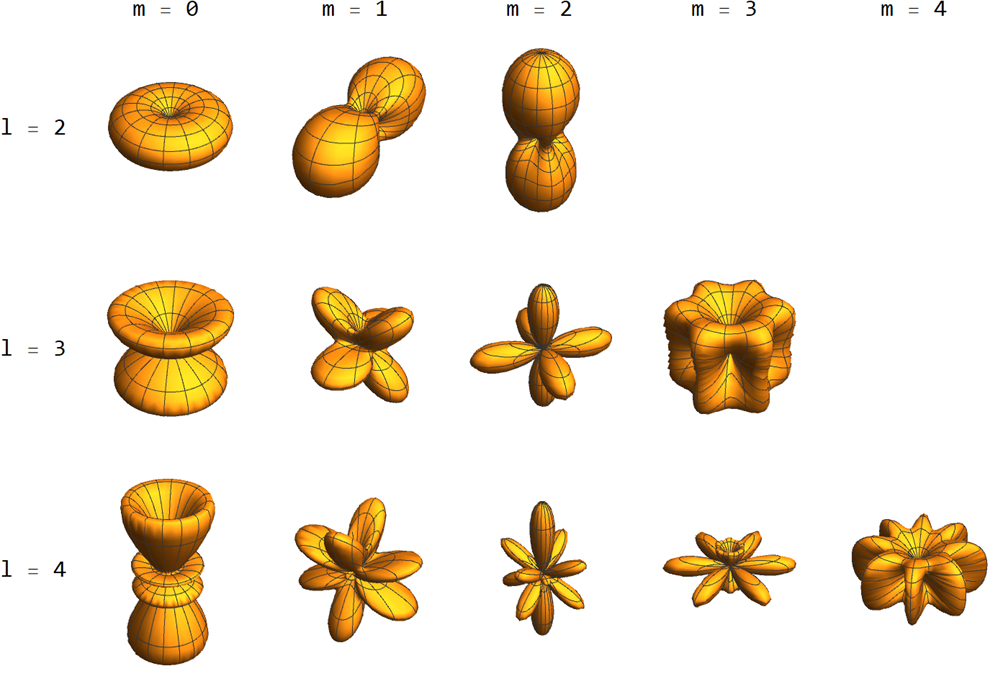
\includegraphics[width=0.8\textwidth]{angle-modes-odd-far}

    \end{frame}

    %
    %
    %
    %%%%%%%%%%%%%%%%%%%%%%%%%%%%%%%%%%%%%%%%%%%%%%%%%%%%%%%%%%%%%%%%%%%%%%%
    %                            FRAME                                    %
    %%%%%%%%%%%%%%%%%%%%%%%%%%%%%%%%%%%%%%%%%%%%%%%%%%%%%%%%%%%%%%%%%%%%%%%
    %
    %
    %

    \begin{frame}\frametitle{Диаграммы направленности (ближняя зона)}

        \centering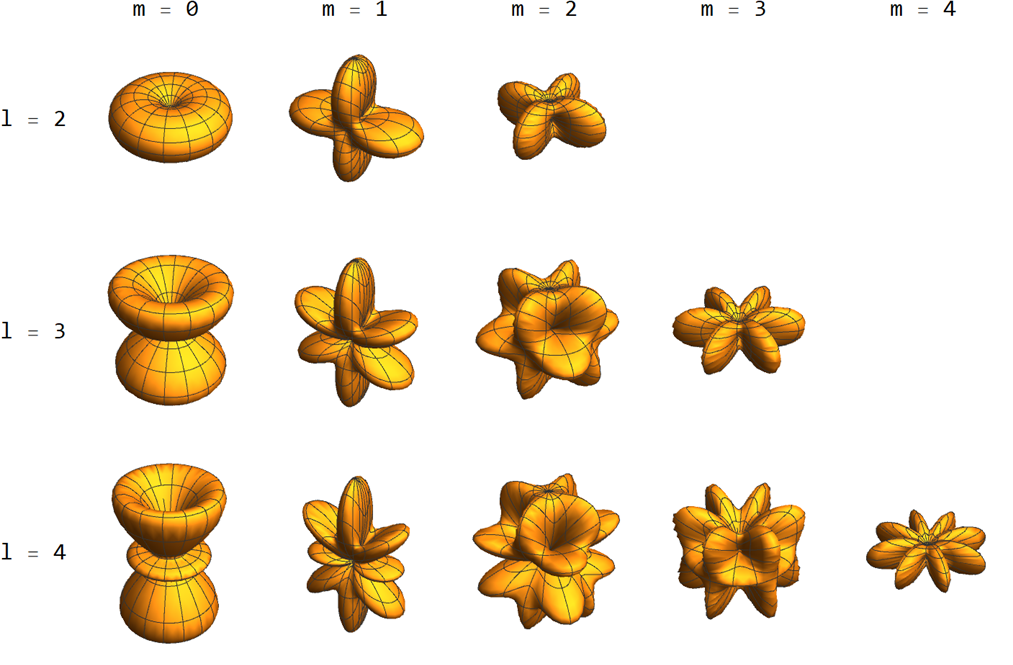
\includegraphics[width=0.8\textwidth]{angle-modes-odd-near}

    \end{frame}

    %
    %
    %
    %%%%%%%%%%%%%%%%%%%%%%%%%%%%%%%%%%%%%%%%%%%%%%%%%%%%%%%%%%%%%%%%%%%%%%%
    %                            FRAME                                    %
    %%%%%%%%%%%%%%%%%%%%%%%%%%%%%%%%%%%%%%%%%%%%%%%%%%%%%%%%%%%%%%%%%%%%%%%
    %
    %
    %

    \begin{frame}\frametitle{Плотность энергии}

        \centering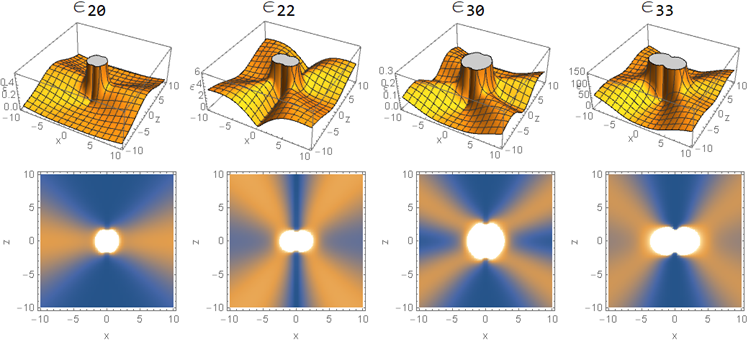
\includegraphics[width=1\textwidth]{energy-odd}

    \end{frame}

    %
    %
    %
    %%%%%%%%%%%%%%%%%%%%%%%%%%%%%%%%%%%%%%%%%%%%%%%%%%%%%%%%%%%%%%%%%%%%%%%
    %                            FRAME                                    %
    %%%%%%%%%%%%%%%%%%%%%%%%%%%%%%%%%%%%%%%%%%%%%%%%%%%%%%%%%%%%%%%%%%%%%%%
    %
    %
    %

    \begin{frame}\frametitle{Поток энергии}

        \begin{figure}[!htb]%
            \centering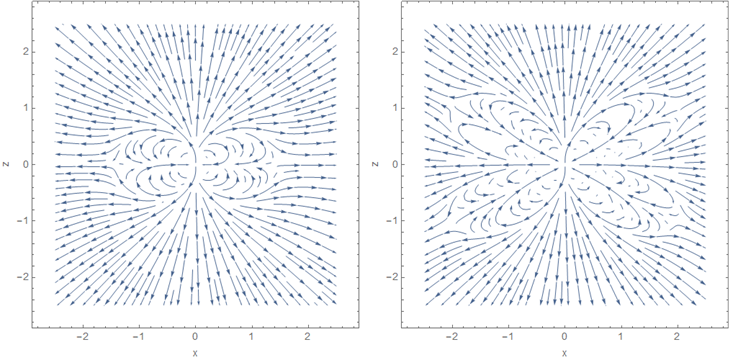
\includegraphics[width=1\textwidth]{pointing-vec-odd}%
            \captionsetup{labelformat=empty}
            \caption[]{Векторные диаграммы потока энергии нечетных базовых мод ($l=2$ и $l=3$) в ближней зоне}
        \end{figure}

    \end{frame}

    %
    %
    %
    %%%%%%%%%%%%%%%%%%%%%%%%%%%%%%%%%%%%%%%%%%%%%%%%%%%%%%%%%%%%%%%%%%%%%%%
    %                            FRAME                                    %
    %%%%%%%%%%%%%%%%%%%%%%%%%%%%%%%%%%%%%%%%%%%%%%%%%%%%%%%%%%%%%%%%%%%%%%%
    %
    %
    %

    \begin{frame}\frametitle{Выводы}

        \begin{itemize}
            \item Описан подход к построению теории гравитации на принципах глобального времени;
            \item Впервые найдены аналитические решения для радиальных частей нечетных мод;
            \item Найдены и исследованы диаграммы направленности нечетных мод в ближней и дальней зонах;
            \item Найдены и исследованы плотность и поток энергии нечетной моды.
        \end{itemize}

    \end{frame}

    %
    %
    %
    %%%%%%%%%%%%%%%%%%%%%%%%%%%%%%%%%%%%%%%%%%%%%%%%%%%%%%%%%%%%%%%%%%%%%%%
    %                            FRAME                                    %
    %%%%%%%%%%%%%%%%%%%%%%%%%%%%%%%%%%%%%%%%%%%%%%%%%%%%%%%%%%%%%%%%%%%%%%%
    %
    %
    %

    \begin{frame}\frametitle{Заключение}

        Кроме исследований характеристик отдельных мод:
        %
        \begin{itemize}
            \item ведутся исследования аппарата симтензорного анализа и бироторного уравнения в общем виде;
            \item более детально анализируется квадратичный лагранжиан;
            \item планируется анализ источников излучения.
        \end{itemize}

    \end{frame}

\end{document}
